\documentclass[14pt]{extbook}
\usepackage{multicol, enumerate, enumitem, hyperref, color, soul, setspace, parskip, fancyhdr} %General Packages
\usepackage{amssymb, amsthm, amsmath, latexsym, units, mathtools} %Math Packages
\everymath{\displaystyle} %All math in Display Style
% Packages with additional options
\usepackage[headsep=0.5cm,headheight=12pt, left=1 in,right= 1 in,top= 1 in,bottom= 1 in]{geometry}
\usepackage[usenames,dvipsnames]{xcolor}
\usepackage{dashrule}  % Package to use the command below to create lines between items
\newcommand{\litem}[1]{\item#1\hspace*{-1cm}\rule{\textwidth}{0.4pt}}
\pagestyle{fancy}
\lhead{Progress Quiz 9}
\chead{}
\rhead{Version C}
\lfoot{9541-5764}
\cfoot{}
\rfoot{Summer C 2021}
\begin{document}

\begin{enumerate}
\litem{
Determine the horizontal and/or oblique asymptotes in the rational function below.\[ f(x) = \frac{6x^{3} -1 x^{2} -75 x + 100}{3x^{2} -14 x + 15} \]\begin{enumerate}[label=\Alph*.]
\item \( \text{Horizontal Asymptote of } y = 2.0  \)
\item \( \text{Horizontal Asymptote at } y = 3.0 \)
\item \( \text{Oblique Asymptote of } y = 2x + 9. \)
\item \( \text{Horizontal Asymptote of } y = 2.0 \text{ and Oblique Asymptote of } y = 2x + 9 \)
\item \( \text{Horizontal Asymptote of } y = 3.0 \text{ and Oblique Asymptote of } y = 2x + 9 \)

\end{enumerate} }
\litem{
Which of the following functions \textit{could} be the graph below?
\begin{center}
    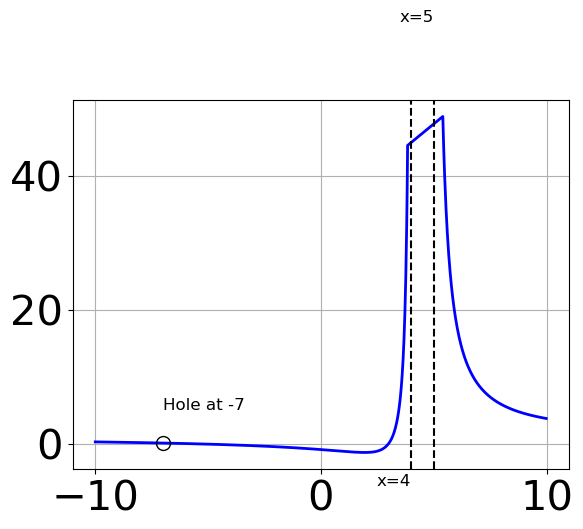
\includegraphics[width=0.5\textwidth]{../Figures/identifyGraphOfRationalFunctionCopyC.png}
\end{center}
\begin{enumerate}[label=\Alph*.]
\item \( f(x)=\frac{x^{3} +5.0 x^{2} -12.0 x -36.0}{x^{3} -2.0 x^{2} -43.0 x + 140.0} \)
\item \( f(x)=\frac{x^{3} -10.0 x^{2} +3.0 x + 126.0}{x^{3} +2.0 x^{2} -43.0 x -140.0} \)
\item \( f(x)=\frac{x^{3} -6.0 x^{2} -9.0 x + 54.0}{x^{3} +2.0 x^{2} -43.0 x -140.0} \)
\item \( f(x)=\frac{x^{3} +10.0 x^{2} +3.0 x -126.0}{x^{3} -2.0 x^{2} -43.0 x + 140.0} \)
\item \( \text{None of the above are possible equations for the graph.} \)

\end{enumerate} }
\litem{
Which of the following functions \textit{could} be the graph below?
\begin{center}
    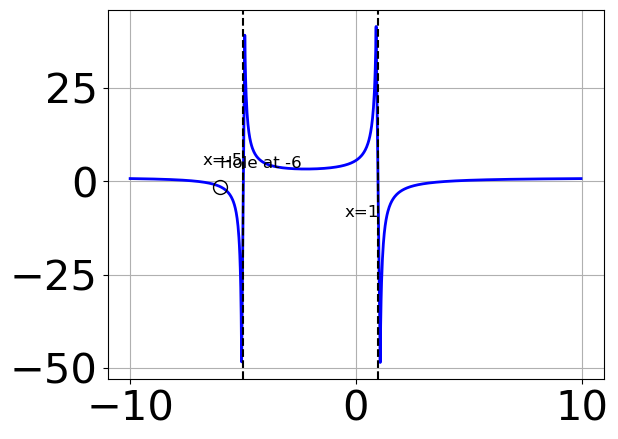
\includegraphics[width=0.5\textwidth]{../Figures/identifyGraphOfRationalFunctionC.png}
\end{center}
\begin{enumerate}[label=\Alph*.]
\item \( f(x)=\frac{x^{3} -2.0 x^{2} -43.0 x + 140.0}{x^{3} +10.0 x^{2} +19.0 x -30.0} \)
\item \( f(x)=\frac{x^{3} + x^{2} -40.0 x -112.0}{x^{3} -10.0 x^{2} +19.0 x + 30.0} \)
\item \( f(x)=\frac{x^{3} +9.0 x^{2} -10.0 x -168.0}{x^{3} +10.0 x^{2} +19.0 x -30.0} \)
\item \( f(x)=\frac{x^{3} -9.0 x^{2} -10.0 x + 168.0}{x^{3} -10.0 x^{2} +19.0 x + 30.0} \)
\item \( \text{None of the above are possible equations for the graph.} \)

\end{enumerate} }
\litem{
Determine the vertical asymptotes and holes in the rational function below.\[ f(x) = \frac{8x^{3} -18 x^{2} -15 x + 25}{6x^{2} -19 x + 10} \]\begin{enumerate}[label=\Alph*.]
\item \( \text{Vertical Asymptotes of } x = 0.667 \text{ and } x = -1.25 \text{ with a hole at } x = 2.5 \)
\item \( \text{Vertical Asymptotes of } x = 0.667 \text{ and } x = 2.5 \text{ with no holes.} \)
\item \( \text{Holes at } x = 0.667 \text{ and } x = 2.5 \text{ with no vertical asymptotes.} \)
\item \( \text{Vertical Asymptote of } x = 0.667 \text{ and hole at } x = 2.5 \)
\item \( \text{Vertical Asymptote of } x = 1.333 \text{ and hole at } x = 2.5 \)

\end{enumerate} }
\litem{
Determine the horizontal and/or oblique asymptotes in the rational function below.\[ f(x) = \frac{20x^{3} -73 x^{2} -34 x + 24}{16x^{3} +44 x^{2} -113 x -60} \]\begin{enumerate}[label=\Alph*.]
\item \( \text{Vertical Asymptote of } y = 4  \)
\item \( \text{Horizontal Asymptote of } y = 0  \)
\item \( \text{Vertical Asymptote of } y = -1.250  \)
\item \( \text{Horizontal Asymptote of } y = 1.250  \)
\item \( \text{None of the above} \)

\end{enumerate} }
\litem{
Determine the vertical asymptotes and holes in the rational function below.\[ f(x) = \frac{9x^{3} -33 x^{2} +10 x + 24}{12x^{2} -x -20} \]\begin{enumerate}[label=\Alph*.]
\item \( \text{Holes at } x = -1.25 \text{ and } x = 1.333 \text{ with no vertical asymptotes.} \)
\item \( \text{Vertical Asymptotes of } x = -1.25 \text{ and } x = 1.333 \text{ with no holes.} \)
\item \( \text{Vertical Asymptote of } x = 0.75 \text{ and hole at } x = 1.333 \)
\item \( \text{Vertical Asymptote of } x = -1.25 \text{ and hole at } x = 1.333 \)
\item \( \text{Vertical Asymptotes of } x = -1.25 \text{ and } x = -0.667 \text{ with a hole at } x = 1.333 \)

\end{enumerate} }
\litem{
Determine the horizontal and/or oblique asymptotes in the rational function below.\[ f(x) = \frac{6x^{3} + x^{2} -11 x -6}{3x^{2} -7 x -6} \]\begin{enumerate}[label=\Alph*.]
\item \( \text{Horizontal Asymptote of } y = 3.0 \text{ and Oblique Asymptote of } y = 2x + 5 \)
\item \( \text{Horizontal Asymptote at } y = 3.0 \)
\item \( \text{Oblique Asymptote of } y = 2x + 5. \)
\item \( \text{Horizontal Asymptote of } y = 2.0 \text{ and Oblique Asymptote of } y = 2x + 5 \)
\item \( \text{Horizontal Asymptote of } y = 2.0  \)

\end{enumerate} }
\litem{
Determine the horizontal and/or oblique asymptotes in the rational function below.\[ f(x) = \frac{15x^{3} +17 x^{2} -46 x -40}{-25x^{3} -20 x^{2} +16 x + 32} \]\begin{enumerate}[label=\Alph*.]
\item \( \text{Vertical Asymptote of } y = 0.800  \)
\item \( \text{Horizontal Asymptote of } y = 0  \)
\item \( \text{Horizontal Asymptote of } y = -0.600  \)
\item \( \text{Vertical Asymptote of } y = -2  \)
\item \( \text{None of the above} \)

\end{enumerate} }
\litem{
Determine the vertical asymptotes and holes in the rational function below.\[ f(x) = \frac{12x^{3} +19 x^{2} -101 x + 60}{6x^{2} -x -15} \]\begin{enumerate}[label=\Alph*.]
\item \( \text{Vertical Asymptotes of } x = -1.5 \text{ and } x = 1.667 \text{ with no holes.} \)
\item \( \text{Holes at } x = -1.5 \text{ and } x = 1.667 \text{ with no vertical asymptotes.} \)
\item \( \text{Vertical Asymptotes of } x = -1.5 \text{ and } x = 0.75 \text{ with a hole at } x = 1.667 \)
\item \( \text{Vertical Asymptote of } x = -1.5 \text{ and hole at } x = 1.667 \)
\item \( \text{Vertical Asymptote of } x = 2.0 \text{ and hole at } x = 1.667 \)

\end{enumerate} }
\litem{
Determine the vertical asymptotes and holes in the rational function below.\[ f(x) = \frac{8x^{3} -34 x^{2} +45 x -18}{8x^{2} -2 x -15} \]\begin{enumerate}[label=\Alph*.]
\item \( \text{Vertical Asymptote of } x = -1.25 \text{ and hole at } x = 1.5 \)
\item \( \text{Vertical Asymptote of } x = 1.0 \text{ and hole at } x = 1.5 \)
\item \( \text{Vertical Asymptotes of } x = -1.25 \text{ and } x = 0.75 \text{ with a hole at } x = 1.5 \)
\item \( \text{Vertical Asymptotes of } x = -1.25 \text{ and } x = 1.5 \text{ with no holes.} \)
\item \( \text{Holes at } x = -1.25 \text{ and } x = 1.5 \text{ with no vertical asymptotes.} \)

\end{enumerate} }
\end{enumerate}

\end{document}